\documentclass[aspectratio=169, 11pt]{beamer}

% ====== Theme ======
\usetheme{Madrid}
\definecolor{CityUBlue}{RGB}{0, 51, 102}
\definecolor{CityULightBlue}{RGB}{0, 102, 179}
\definecolor{CityUGold}{RGB}{198, 163, 0}
\usecolortheme[named=CityUBlue]{structure}
\setbeamercolor{title}{fg=white, bg=CityUBlue}
\setbeamercolor{frametitle}{fg=white, bg=CityUBlue}
\setbeamercolor{block title}{bg=CityUBlue, fg=white}
\setbeamercolor{block body}{bg=CityUBlue!10, fg=black}
\setbeamercolor{item}{fg=CityUBlue}
\setbeamercolor{subitem}{fg=CityULightBlue}

% ====== Packages ======
\usepackage[T1]{fontenc}
\usepackage{lmodern}
\usepackage{booktabs}
\usepackage{graphicx}
\usepackage{hyperref}
\usepackage{amsmath, amssymb}
\usepackage{tikz}
\usepackage{appendixnumberbeamer}

% ====== Settings ======
\setbeamertemplate{navigation symbols}{}
\graphicspath{{figures/}{../../Figures used in slides/}}

% ====== Metadata ======
\title[EF8083 Lecture 5]{PhD Lecture in Behavioral Asset Pricing:\\ Bounded Rationality and Psychology-free Models}
\author[F.\ W.\ Li]{Frank Weikai Li}
\institute[CityU]{Associate Professor of Finance\\City University of Hong Kong}
\date{}

% ==============================================================================
\begin{document}
% ==============================================================================

% --- Slide 1: Title ---
\begin{frame}[plain]
\titlepage
\end{frame}

% --- Slide 2: Overview ---
\section{Overview}

\begin{frame}{Overview}
\begin{itemize}
\item \textbf{Bounded rationality:} people get only complicated or subtle things wrong
  \begin{itemize}
  \item Broad theme: we have limited capacity for gathering and processing information
  \end{itemize}
\item \textbf{Specific topics:}
  \begin{itemize}
  \item \textbf{Limited attention}
    \begin{itemize}
    \item Underreaction to news
    \item Buying vs.\ selling decisions of individual investors
    \item Causal effect of attention on asset prices
    \end{itemize}
  \item \textbf{Category thinking}
  \end{itemize}
\item \textbf{Psychology-free models:} we can make interesting predictions without explicit use of psychological concepts
  \begin{itemize}
  \item Actions of sophisticated traders
  \item Actions of noise traders
  \item Impacts of investor sentiment (equity and credit market sentiment)
  \end{itemize}
\end{itemize}
\end{frame}

% --- Slide 3: Limited Attention I ---
\section{Limited Attention}

\begin{frame}{}
\vfill
\centering
{\Large \textbf{Limited Attention}}
\vfill
\end{frame}

\begin{frame}{Limited Attention I}
\begin{itemize}
\item \textbf{Theme:}
  \begin{itemize}
  \item Because of limited attention, investors may underreact to news
  \end{itemize}
\item \textbf{Underreaction to earnings news}
  \begin{itemize}
  \item Limited attention predicts weaker immediate market reaction and stronger post-earnings announcement drift (PEAD)
  \end{itemize}
\item \textbf{Two influential studies:}
  \begin{itemize}
  \item PEAD is stronger for firms that announce earnings at the same time as many other firms (Hirshleifer, Lim, and Teoh, 2009)
  \item PEAD is stronger for firms that announce earnings on Friday (Della Vigna and Pollet, 2009)
  \item These two studies help rule out the alternative explanation that the differential PEAD is due to differential information content of earnings surprises
  \end{itemize}
\end{itemize}
\end{frame}

% --- Slide 4: Limited Attention I ctd ---
\begin{frame}{Limited Attention I, ctd.}
\begin{columns}[T]
\begin{column}{0.34\textwidth}
\centering
\includegraphics[width=\textwidth]{figures/Friday_EA.png}
\end{column}
\begin{column}{0.62\textwidth}
\vspace{1.5em}
{\footnotesize \textbf{Della Vigna and Pollet (2009)}: Friday earnings announcements exhibit a \emph{weaker immediate market reaction} but a \emph{stronger post-earnings announcement drift (PEAD)} than announcements on other days.}
\end{column}
\end{columns}
\end{frame}

% --- Slide 5: Frog in the Pan ---
\begin{frame}{Limited Attention I, ctd.}
\begin{itemize}
\item \textbf{A potential explanation for momentum} (Da, Gurun, and Warachka, 2014)
  \begin{itemize}
  \item A series of frequent small changes attracts less attention than infrequent large changes
  \item ``Frog in the Pan'' hypothesis: investors are more likely to be inattentive to information arriving continuously in small amounts than to information that arrives in large amounts at discrete time points
  \item Momentum is stronger when information arrives continuously as opposed to discretely
  \end{itemize}
\end{itemize}
\vfill
\centering
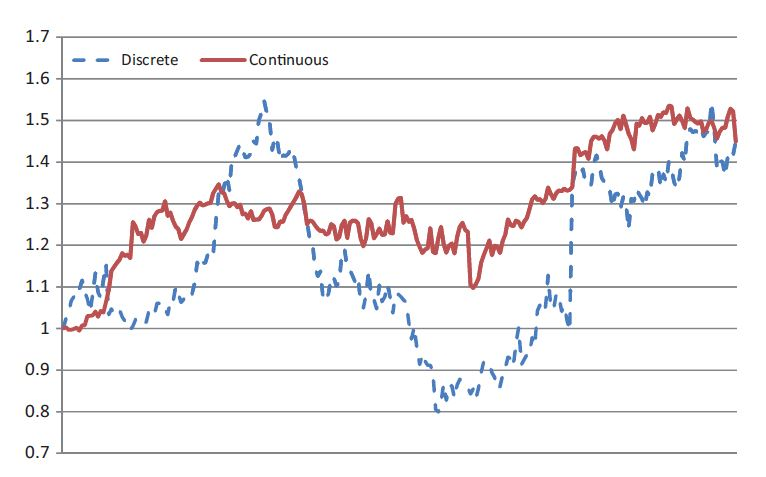
\includegraphics[width=0.45\textwidth]{figures/slide05_pic4.jpg}%
\hspace{0.6em}%
\end{frame}

% --- Slide 6: Underreaction to subtle news ---
\begin{frame}[shrink=5]{Limited Attention I, ctd.}
\begin{itemize}
\item Underreaction is more likely to occur when the news is \textbf{less salient or more subtle} 
\item \textbf{Underreaction to demographic information}
  \begin{itemize}
  \item Della Vigna and Pollet (2008): investors are slow to recognize the impact of demographic shifts on the future profitability of firms with age-sensitive products
  \item E.g.\ Baby boom today predicts higher demand for toys in 6 years, so prices of toy-making firms should rise immediately in an efficient market
  \end{itemize}
\item \textbf{Underreaction to technological information}
  \begin{itemize}
  \item Innovative efficiency: Hirshleifer, Hsu, and Li (2013)
  \item Track records in innovation ability: Cohen, Diether, and Malloy (2013)
  \end{itemize}
\item \textbf{Underreaction to the absence of news: No news is news}
  \begin{itemize}
  \item Giglio and Shue (2014): investors underreact to the probability of merger deal completion contained in the passage of time
  \end{itemize}
\end{itemize}
\end{frame}

% --- Slide 6a: Instructor's research ---
\begin{frame}[shrink=5]{My Research: The Information Content of Sudden Insider Silence}
\begin{itemize}
\item \textbf{Hong and Li (JFQA 2019)}, ``The Information Content of Sudden Insider Silence'' 
  \begin{itemize}
  \item Identifies ``routine'' insiders from their calendar trading patterns
  \item Sudden silence is a deviation from routine trading patterns
  \item Routine insiders strategically stay silent when they hold private information
  \item Silence after routine selling (buying) predicts positive (negative) future returns and fundamentals
  \item A long-short strategy earns 6--10\% annually
  \item Returns concentrate at earnings announcements and are stronger where information environments are poor and arbitrage is costly
  \end{itemize}
\item \textbf{Connection:} the previous slide shows investors underreact to subtle news; here they underreact to the \emph{absence} of an expected event, because it is hard to recognize that nonoccurrence can be informative
\end{itemize}
\end{frame}

% --- Slide 7: Momentum Spillover ---
\begin{frame}{Limited Attention I, ctd.}
\begin{columns}
\begin{column}{0.5\textwidth}
\begin{itemize}
\item A growing literature documents that investors underreact to news of economically linked peers (``momentum spillover effect'')
\item \textbf{Customer-Supplier Links} (Cohen and Frazzini, 2008)
  \begin{itemize}
  \item Firms are required to report their major customers ($>$10\% of sales)
  \item Investors are slow to recognize that good news for a customer is good news for the supplier
  \end{itemize}
\end{itemize}
\end{column}
\begin{column}{0.48\textwidth}
\centering
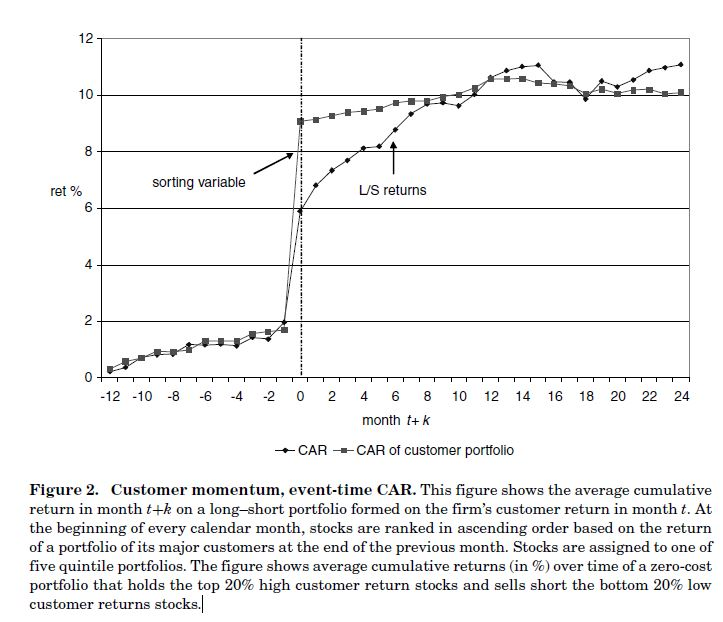
\includegraphics[width=\linewidth]{figures/slide07_pic4.jpg}\\[0.2em]
\footnotesize Cohen and Frazzini (2008)
\end{column}
\end{columns}
\end{frame}

% --- Slide 8: Other Economic Linkages ---
\begin{frame}[shrink=5]{Limited Attention I, ctd.}
\begin{itemize}
\item The same pattern holds for other types of economic linkages
\item \textbf{Industry and product market peers}
  \begin{itemize}
  \item Moskowitz and Grinblatt (1999): firms operating in the same industry (industry momentum)
  \item Cohen and Lou (2012): conglomerate firms are slower than standalone firms to reflect industry news
  \item Huang (2015): stock prices of multinational firms underreact to foreign industry news
  \item Hoberg and Phillips (2016): product market peers identified through annual reports
  \end{itemize}
\item \textbf{Geographic peers}
  \begin{itemize}
  \item Parsons, Sabbatucci, and Titman (2020): firms headquartered in the same state
  \item Jin and Li (2024): firms with overlapping geographic establishments
  \end{itemize}
\item \textbf{Technological peers}
  \begin{itemize}
  \item Lee et al.\ (2018): firms sharing the same type of technologies
  \end{itemize}
\item \textbf{Analyst co-coverage}
  \begin{itemize}
  \item Ali and Hirshleifer (2019): firms followed by the same set of analysts
  \end{itemize}
\end{itemize}
\end{frame}

% --- Slide 8a: Instructor's research ---
\begin{frame}[shrink=5]{My Research: Geographic and Scope Links}
\begin{itemize}
\item \textbf{Jin and Li (JBFA 2024), geographic links}
  \begin{itemize}
  \item Links firms through overlapping establishment locations (where sales are generated), not headquarters
  \item Returns of geography-linked peers predict focal-firm returns and fundamentals
  \item The effect is stronger for low-attention firms, costly-to-arbitrage stocks, and during high-sentiment periods
  \end{itemize}
\item \textbf{Jin and Li (working paper), scope similarity}
  \begin{itemize}
  \item Links firms through Hoberg--Phillips product-market scope that transcends industry boundaries; investors are slow to incorporate news about scope peers, and a long-short portfolio earns 8.9\% per year in five-factor alpha
  \end{itemize}
\item \textbf{Connection:} the momentum-spillover evidence on the previous slides relies on named linkages (customers, industries); here the linkage itself is the subtle information investors fail to process
\end{itemize}
\end{frame}

% --- Slide 9: Cross-Asset Predictability ---
\begin{frame}{Limited Attention I, ctd.}
\begin{columns}
\begin{column}{0.5\textwidth}
\begin{itemize}
\item Several papers document significant return predictability across debt and equity securities of the same firm
\item Han, Subrahmanyam, and Zhou (JFE 2017)
  \begin{itemize}
  \item The term structure of firms' credit spreads predicts future firm fundamentals and stock returns
  \end{itemize}
\item Addoum and Murfin (RFS 2020)
  \begin{itemize}
  \item Prices of syndicated loans contain useful information for equity prices but investors fail to unravel such information, leading to return predictability from the loan market to the equity market
  \end{itemize}
\end{itemize}
\end{column}
\begin{column}{0.48\textwidth}
\centering

\includegraphics[width=\linewidth]{figures/slide09_pic4.png}\\[0.2em]
\footnotesize Addoum and Murfin (RFS 2020)
\end{column}
\end{columns}
\end{frame}

% --- Slide 10: Market Segmentation ---
\begin{frame}{Limited Attention I, ctd.}
\begin{itemize}
\item The source of underreaction could be ``market segmentation''
  \begin{itemize}
  \item Both debt and equity are claims to the same underlying cash flows/asset values
  \item Investors trading in debt markets have low overlap with those trading in equity markets, leading to underreaction to cross-asset information
  \item Supporting this explanation, the returns to cross-asset momentum are lower among equities held by mutual funds also trading in debt securities (dual ownership) 
  \end{itemize}
\end{itemize}
\end{frame}

% --- Slide 11: Other Asset Classes ---
\begin{frame}{Limited Attention I, ctd.}
\begin{columns}
\begin{column}{0.5\textwidth}
\begin{itemize}
\item Firm value is also affected by shocks to other asset classes, including currencies and commodities
\item \textbf{Cross-asset return predictability}
\item Bae, Da, and Zurita (2023)
  \begin{itemize}
  \item Equity investors of U.S.\ multinationals underreact to firms' currency shocks from the countries in which they operate
  \end{itemize}
\item Ho and Lauwers (2023)
  \begin{itemize}
  \item Aggregate positions of traders in the commodity futures market can predict the cross-section of stock returns for commodity producers
  \end{itemize}
\end{itemize}
\end{column}
\begin{column}{0.48\textwidth}
\centering
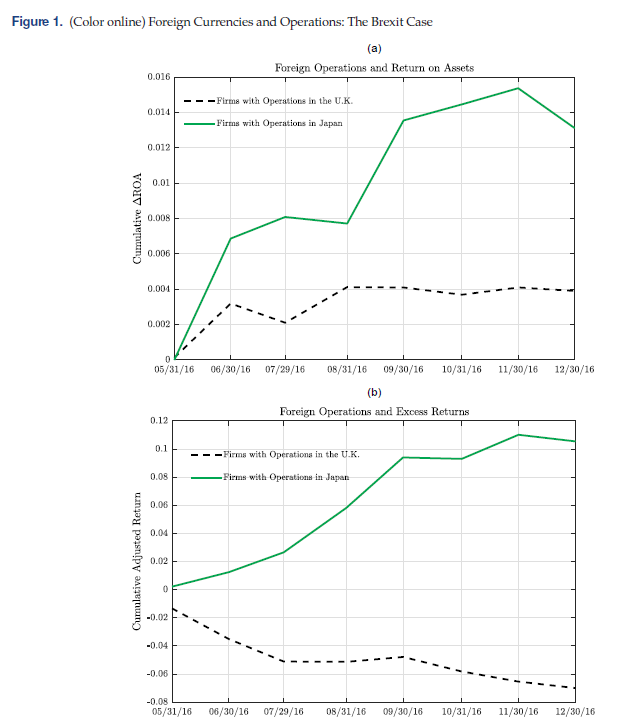
\includegraphics[width=\linewidth,height=0.75\textheight,keepaspectratio]{figures/slide11_pic4.png}\\[0.2em]
\footnotesize Ho and Lauwers (2023)
\end{column}
\end{columns}
\end{frame}

% --- Slide 12: Limited Attention II ---
\begin{frame}[shrink=5]{Limited Attention II}
\begin{itemize}
\item \textbf{Theme:}
  \begin{itemize}
  \item Attention is more important for individual investors' buying decisions than for their selling decisions (Why?)
  \item Barber and Odean (2008) show that there is indeed stronger buying interest than selling interest, among individual investors, for attention-grabbing stocks
  \item Measure attention with extreme returns, high volume, or news announcements
  \end{itemize}
\end{itemize}
\vfill
\centering
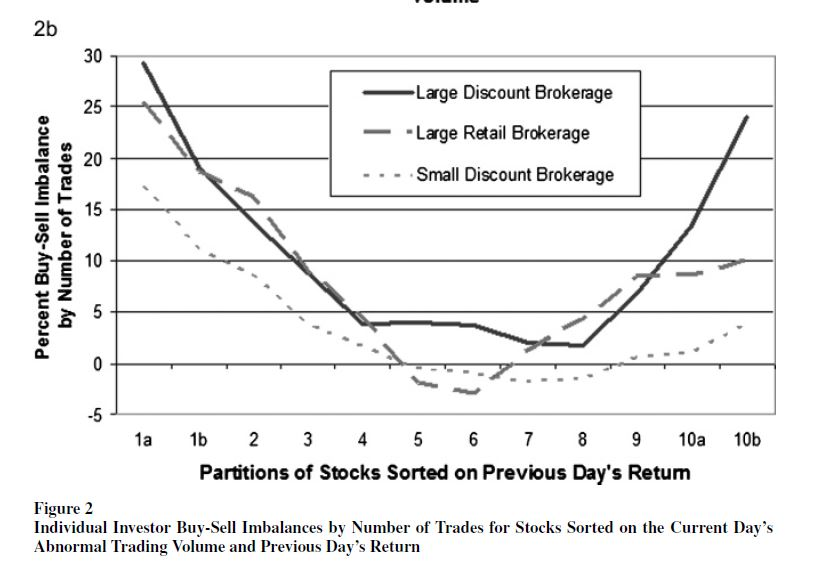
\includegraphics[width=0.50\textwidth]{figures/slide12_pic4.jpg}
\end{frame}

% --- Slide 13: Limited Attention III ---
\begin{frame}{Limited Attention III}
\begin{itemize}
\item Because of limited processing capacity, investors may only pay attention to one kind of information
\item \textbf{Hong and Stein (1999)}
\item Two types of investors:
  \begin{itemize}
  \item Newswatchers, who only process private information
  \item Momentum traders, who only track past prices, and whose demand is a function of the past price change
  \end{itemize}
\item Assume that private information diffuses slowly through the newswatcher population
  \begin{itemize}
  \item In an economy with only newswatchers, this would generate momentum
  \end{itemize}
\item In an economy with both kinds of investors, we can generate both momentum and long-term reversals
  \begin{itemize}
  \item It is optimal for momentum traders' demand to be a positive function of the past price change
  \item Price eventually overshoots because momentum traders keep buying even after (positive) private information is fully incorporated into prices
  \end{itemize}
\end{itemize}
\end{frame}

% --- Slide 14: Hong Lim Stein ---
\begin{frame}{Limited Attention III, ctd.}
\begin{itemize}
\item Hong, Lim, and Stein (2000)
\item Test the Hong and Stein (1999) hypothesis that momentum is due to slow infusion of private information
  \begin{itemize}
  \item They find that momentum is stronger among small stocks and stocks with low analyst coverage
  \end{itemize}
\end{itemize}
\vfill
\centering
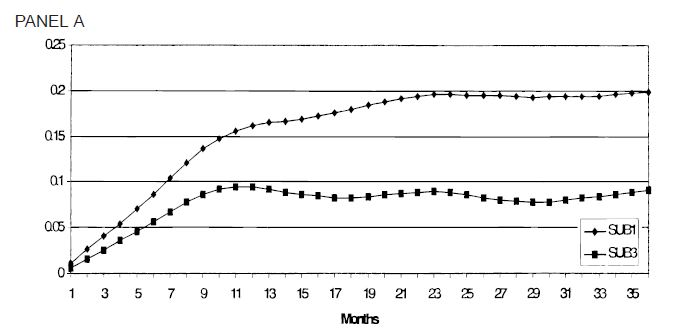
\includegraphics[width=0.55\textwidth]{figures/slide14_pic4.jpg}
\end{frame}

% --- Slide 15: Causal Effect of Attention ---
\begin{frame}{Causal Effect of Attention on Asset Prices}
\begin{columns}
\begin{column}{0.5\textwidth}
\begin{itemize}
\item The key challenge in identifying the causal effect of attention on asset prices is that investor attention is endogenous to stock fundamentals (possibly unobservable)
\item Chen, An, Wang, and Yu (JF 2023) circumvent this issue by exploring the attention spillover effect
\item They exploit the unique setting in China where the on-screen display order of stocks is determined by the stock's listing code
\item Investors are more likely to pay attention to neighboring stocks if they have positive investment experience with the focal stock
\end{itemize}
\end{column}
\begin{column}{0.48\textwidth}
\centering
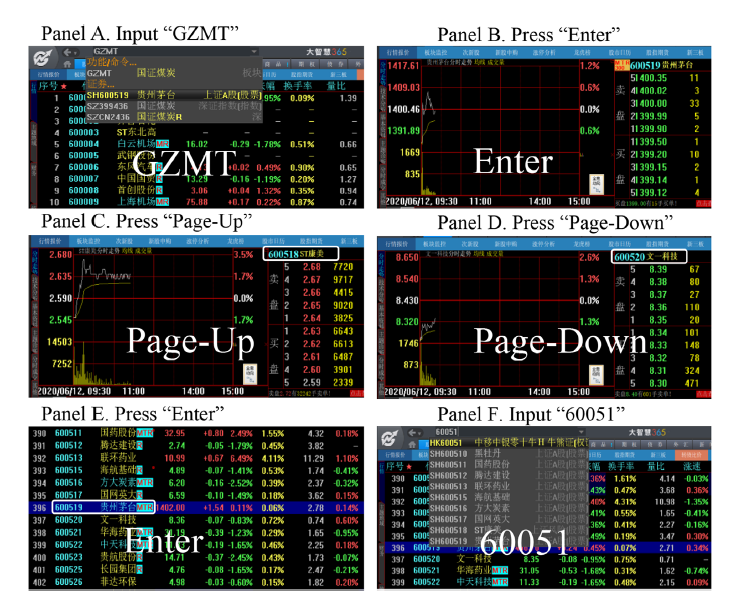
\includegraphics[width=\linewidth]{figures/slide15_pic4.png}\\[0.2em]
\footnotesize Chen, An, Wang, and Yu (JF 2023)
\end{column}
\end{columns}
\end{frame}

% --- Slide 16: Causal Evidence ---
\begin{frame}{Causal Effect of Attention on Asset Prices, ctd.}
\begin{columns}
\begin{column}{0.5\textwidth}
\begin{itemize}
\item Because attention leads to excessive buying demand, stocks displayed next to those with higher returns in the past two weeks are associated with higher returns in the following week, which revert in the long run
\end{itemize}
\end{column}
\begin{column}{0.48\textwidth}
\centering
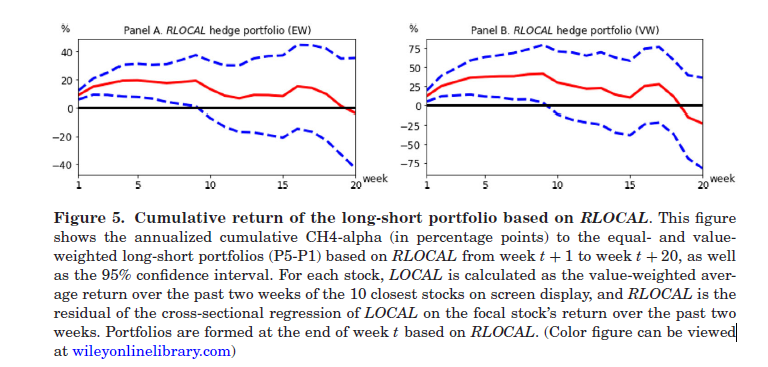
\includegraphics[width=\linewidth]{figures/slide16_pic4.png}\\[0.2em]
\footnotesize Chen, An, Wang and Yu (JF 2023)
\end{column}
\end{columns}
\end{frame}

% --- Slide 17: Section ---
\section{Category Thinking}

\begin{frame}{}
\vfill
\centering
{\Large \textbf{Category Thinking}}
\vfill
\end{frame}

% --- Slide 18: Category Thinking ---
\begin{frame}{Category Thinking}
\begin{itemize}
\item A basic feature of the way humans think about a complex world is that we put things into categories and form beliefs at the level of these categories (Rosch and Lloyd, 1978)
\item It is plausible that such category-based thinking also applies to investment
  \begin{itemize}
  \item As there are thousands of individual securities and funds, investors may simplify their decision-making by putting financial assets into categories
  \item We often use labels such as ``value stocks,'' ``growth stocks,'' ``small-cap stocks''
  \end{itemize}
\item \textbf{Barberis and Shleifer (2003)}
  \begin{itemize}
  \item Model where some investors put assets into categories and form beliefs about the assets' future returns at the category level
  \end{itemize}
\item A novel prediction is \textbf{excess return comovement}
  \begin{itemize}
  \item Returns of assets in the same category comove more than can be explained by fundamentals, driven by correlated demand shocks
  \end{itemize}
\end{itemize}
\end{frame}

% --- Slide 19: Evidence for Category Thinking ---
\begin{frame}{Category Thinking, ctd.}
\begin{itemize}
\item Numerous studies document excess return comovement among firms or funds sharing similar characteristics, supporting Barberis and Shleifer (2003):
  \begin{itemize}
  \item Stocks belonging to the same indices (Barberis et al., 2005; Greenwood, 2008; Boyer, 2011)
  \item Firms headquartered in the same state (Pirinsky and Wang, 2006)
  \item Stocks with similar levels of prices (Green and Hwang, 2009)
  \item Firms covered by similar sets of analysts (Israelsen, 2016)
  \item Stocks held by a common set of mutual funds (Anton and Polk, 2014)
  \item Dividend-paying stocks (Hameed and Xie, 2019)
  \end{itemize}
\end{itemize}
\end{frame}

% --- Slide 20: S&P 500 Comovement ---
\begin{frame}{Excess Return Comovement among Stocks in the Same Index}
\begin{itemize}
\item Barberis, Shleifer, and Wurgler (2005) test the prediction of category thinking that a stock that is added to (removed from) the S\&P 500 index will experience a large increase (decrease) in its loading on the S\&P return
\[
R_{j,t} = \alpha_j + \beta_{j,\text{SP500}}\, R_{\text{SP500},t} + \beta_{j,\text{nonSP500}}\, R_{\text{nonSP500},t} + v_{j,t}
\] 
\end{itemize}
\vfill
\centering
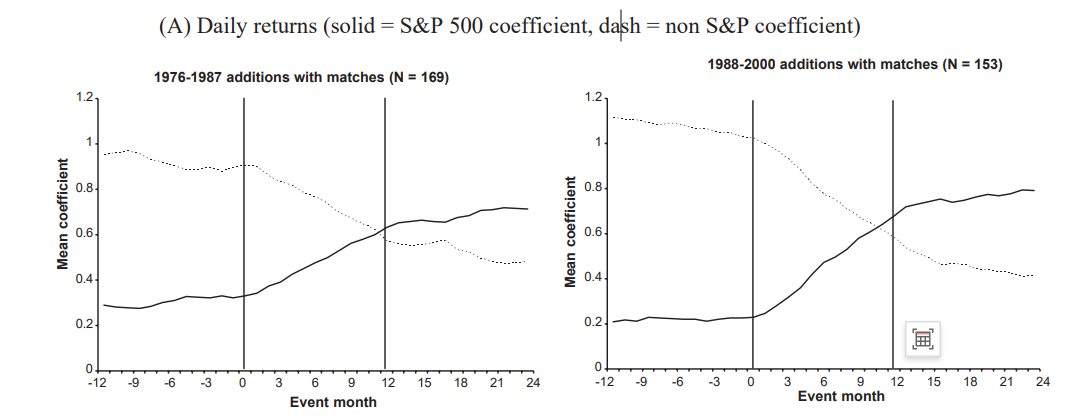
\includegraphics[width=0.60\textwidth]{figures/slide20_pic4.png}
\end{frame}

% --- Slide 21: Section ---
\section{Psychology-free Approaches}

\begin{frame}{}
\vfill
\centering
{\Large \textbf{Psychology-free Approaches}}
\vfill
\end{frame}

% --- Slide 22: Psychology-free Approaches ---
\begin{frame}[shrink=5]{Psychology-free Approaches}
\begin{itemize}
\item The approaches discussed so far have mostly been rooted in a psychological concept
\item Some behavioral finance models shed light on the asset pricing facts without appealing to any specific psychology
\item A common structure for such a model is De Long et al.\ (1990), where less than fully rational investors (``noise traders'') interact with more rational traders known as ``arbitrageurs''
\item Even without additional psychological assumptions, it yields many testable predictions:
  \begin{itemize}
  \item The level of mispricing will be higher for assets whose valuation is more uncertain
  \item The level of mispricing will be higher for assets whose characteristics make arbitrage more difficult
  \item Arbitrageurs' actions in correcting mispricing are informative about future asset returns
  \end{itemize}
\end{itemize}
\end{frame}

% --- Slide 23: Sophisticated Agents ---
\begin{frame}[shrink=5]{Actions of Sophisticated Agents}
\begin{itemize}
\item If some assets are mispriced, the trades of sophisticated investors should predict returns
\item \textbf{Who are these sophisticated investors?}
\item \textbf{Firm managers}
  \begin{itemize}
  \item The key assumption is that firm managers can detect and respond to market mispricing
  \item Issuance/repurchase decisions: change the supply of shares in response to investor demand
  \item Personal transactions in their own firms' stocks --- ``corporate insider trading''
  \end{itemize}
\item \textbf{Short sellers}
  \begin{itemize}
  \item Stocks heavily shorted have low subsequent returns (Asquith, Pathak, and Ritter, 2005)
  \end{itemize}
\item \textbf{Hedge funds}
  \begin{itemize}
  \item Chen, Da, and Huang (2018): net arbitrage trading (NAT) of hedge funds strongly predicts stock returns in the cross-section
  \end{itemize}
\item \textbf{Analysts?}
  \begin{itemize}
  	\item Most studies show analyst recommendations and price targets are biased and overly optimistic
    \item Lee and So (2017) show that abnormal analyst coverage positively predicts subsequent return
    \item Look at what analysts do, not what they say 
  \end{itemize}
\end{itemize}
\end{frame}

% --- Slide 24: Aggregate Predictions ---
\begin{frame}[shrink=5]{Actions of Sophisticated Agents, ctd.}
\begin{itemize}
\item Interestingly, actions of sophisticated investors, when aggregated to the market level, can predict market returns in the same direction as stock-level returns
  \begin{itemize}
  \item Baker and Wurgler (2000): the share of equity issues in total equity and debt issues negatively predicts market returns
  \item Seyhun (1988): aggregate trading by corporate insiders positively predicts future market returns
  \item Rapach, Ringgenberg, and Zhou (2016): aggregate short interest negatively forecasts market returns
  \end{itemize}
\end{itemize}
\vfill
\centering
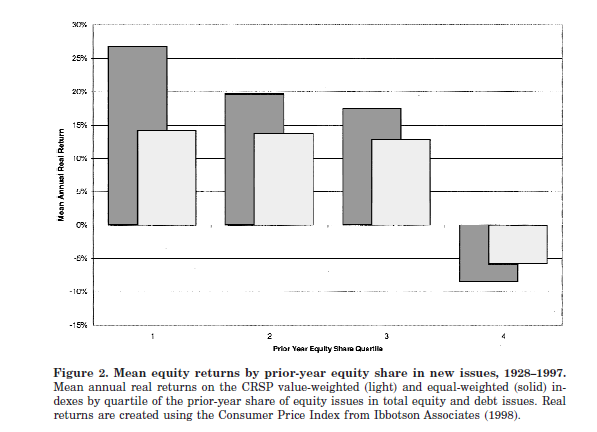
\includegraphics[width=0.50\textwidth]{figures/slide24_pic3.png}\\[0.2em]
\footnotesize Baker and Wurgler (2000)
\end{frame}

% --- Slide 25: Noise Traders ---
\begin{frame}{Actions of Noise Traders}
\begin{itemize}
\item If some assets are mispriced, the trades and actions of unsophisticated agents should negatively predict returns
\item \textbf{Several studies confirm this:}
\item \textbf{Frazzini and Lamont (2008)}
  \begin{itemize}
  \item Stocks held by mutual funds with large inflows in the previous three years have low subsequent returns
  \end{itemize}
\item \textbf{Barber, Odean, and Zhu (2008) and Hvidkjaer (2008)}
  \begin{itemize}
  \item Stocks heavily bought by individual investors in the previous year perform poorly in the following year
  \item Use small trades in the TAQ dataset to identify individuals and the Lee-Ready algorithm to identify buy/sell orders
  \end{itemize}
\item \textbf{Da, Engelberg, and Gao (2011)}
  \begin{itemize}
  \item Higher investor attention as captured by Google search volume is correlated with abnormal retail buying and leads to elevated stock price initially but lower returns over the long run
  \end{itemize}
\end{itemize}
\end{frame}


% --- Slide 36a: Instructor's research ---
\begin{frame}[shrink=5]{My Research: Information Acquisition via EDGAR Search}
	\begin{itemize}
		\item \textbf{Li and Sun (JEDC 2022)}
		\begin{itemize}
			\item SEC EDGAR server logs record the number of IP addresses searching each firm's filings, a direct measure of costly information acquisition
			\item Abnormal EDGAR search predicts future returns and fundamentals
			\item A long-short portfolio earns 80 bps monthly with no long-run reversal
			\item Predictability is stronger for larger and lengthier filings that cost more to process, consistent with endogenous information acquisition
		\end{itemize}
		\item \textbf{Connection:} Google search volume measures what grabs retail investors' attention; EDGAR search measures deliberate, costly processing by sophisticated investors. The two behave oppositely: attention-driven demand reverses, informed acquisition does not
	\end{itemize}
\end{frame}

% --- Slide 26: Baker Wurgler Sentiment ---
\section{Investor Sentiment}

\begin{frame}{}
\vfill
\centering
{\Large \textbf{Investor Sentiment}}
\vfill
\end{frame}

\begin{frame}[shrink=5]{Market-based Measures of Sentiment}
\begin{itemize}
\item Baker and Wurgler (2006)
\item Measure investor ``sentiment'' using the principal component of the following six proxies from market data:
  \begin{itemize}
  \item \textbf{Trading volume:} TURN is defined as the natural logarithm of the ratio of NYSE trading volume to the number of shares listed, detrended by the 5-year moving average
  \item \textbf{Closed-end fund discount:} CEFD is defined as the average difference between the net asset values of closed-end stock fund shares and their market prices
  \item \textbf{IPO activity:} NIPO is defined as the number of IPOs
  \item \textbf{First-day returns:} RIPO is defined as the average of first-day returns on IPOs
  \item \textbf{Equity issues:} S is defined as the ratio of gross equity issuance to the sum of gross equity and gross long-term debt issuance by all corporations
  \item \textbf{Dividend premium:} DP is defined as the difference between the average market-to-book ratios of dividend payers and nonpayers
  \end{itemize}
\item Each of those measures has been proposed by prior studies as capturing investor sentiment
\end{itemize}
\end{frame}

% --- Slide 27: BW Index ---
\begin{frame}[shrink=5]{Baker and Wurgler Sentiment Index}
\vfill
\centering
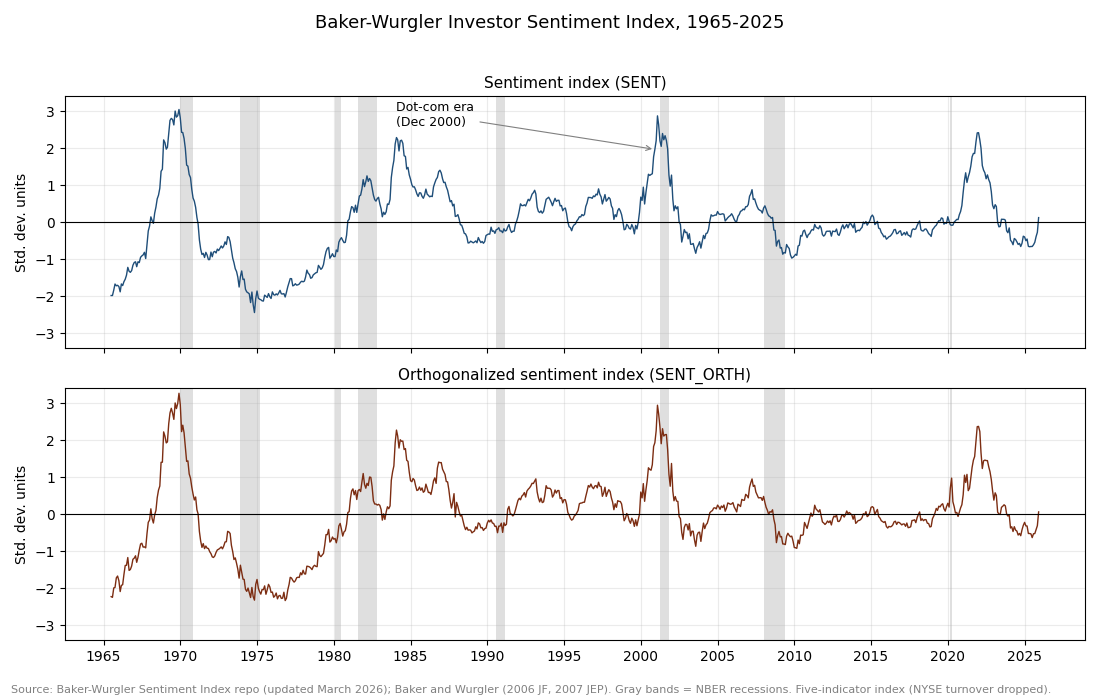
\includegraphics[width=0.80\textwidth]{figures/BW_sentiment_index.png}\\[0.2em]
\footnotesize Source: Baker and Wurgler (2006); Huang, Jiang, Tu, and Zhou (2015)
\vfill
\end{frame}

% --- Slide 28: PLS Index ---
\begin{frame}{Baker and Wurgler Sentiment Index}
\begin{columns}
\begin{column}{0.5\textwidth}
\begin{itemize}
\item Huang, Jiang, Tu, and Zhou (2015)
\item Refine the BW sentiment index by using the partial least squares (PLS) regression to more efficiently extract the return forecasting information from the six underlying proxies
\item They show the new index has much greater predictive power than the original sentiment indices, both in and out of sample
\end{itemize}
\end{column}
\begin{column}{0.48\textwidth}
\centering
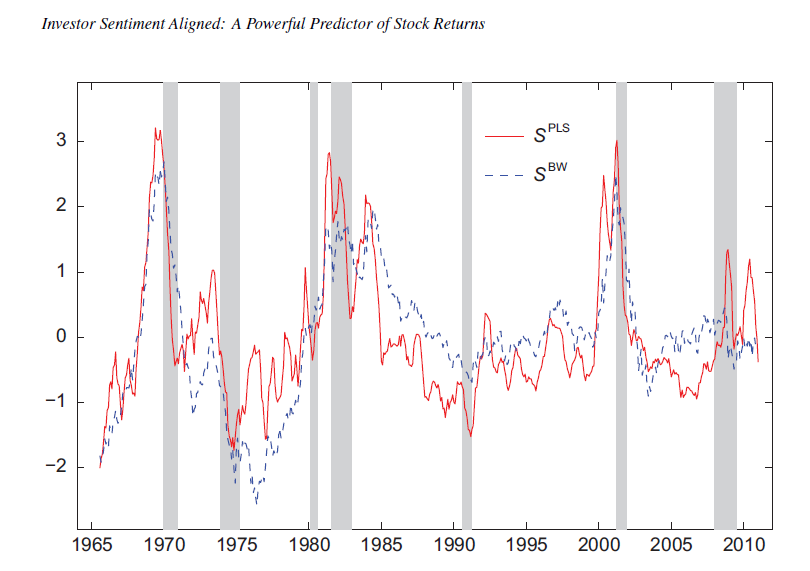
\includegraphics[width=\linewidth]{figures/slide28_pic4.png}\\[0.2em]
\footnotesize Huang, Jiang, Tu, and Zhou (2015)
\end{column}
\end{columns}
\end{frame}

% --- Slide 29: Sentiment and Market Returns ---
\begin{frame}{Effects of Investor Sentiment on the Stock Market (I)}
\begin{itemize}
\item Baker and Wurgler (2007): Sentiment should predict market returns with a negative sign
\end{itemize}
\vfill
\centering
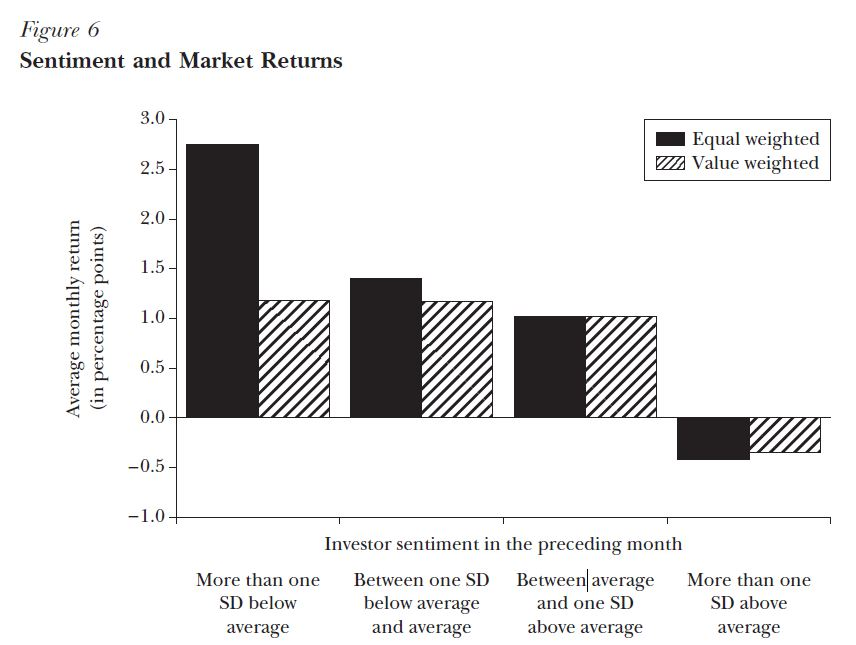
\includegraphics[width=0.55\textwidth]{figures/slide29_pic4.jpg}
\end{frame}

% --- Slide 30: Role of Uncertainty ---
\begin{frame}{Effects of Investor Sentiment on the Stock Market (I) --- Role of Uncertainty}
\begin{columns}
\begin{column}{0.5\textwidth}
\begin{itemize}
\item Birru and Young (JFE 2022) show that the return predictability of investor sentiment is much greater when uncertainty is high
\item This is consistent with the idea that sentiment exhibits its strongest effects on asset prices at times when valuations are most subjective
\end{itemize}
\end{column}
\begin{column}{0.48\textwidth}
\centering
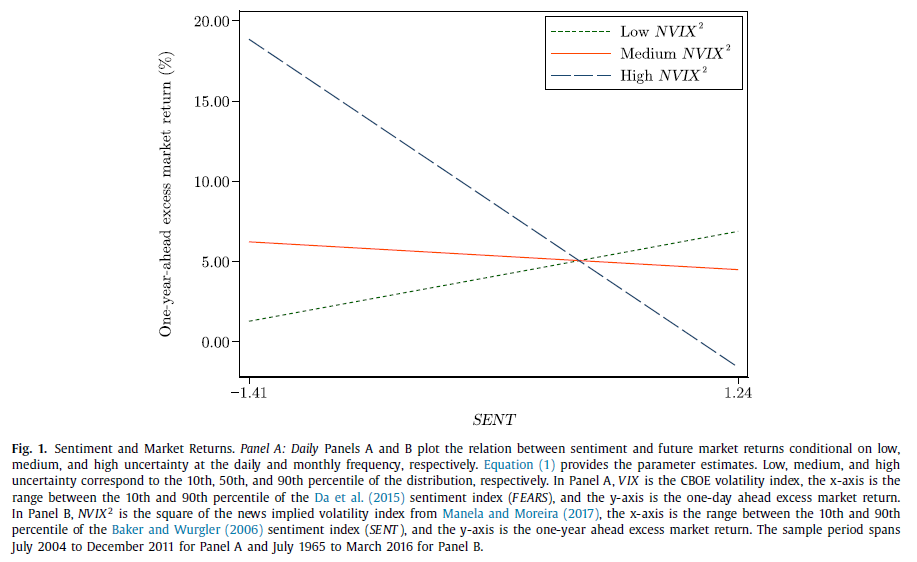
\includegraphics[width=\linewidth]{figures/slide30_pic4.png}\\[0.2em]
\footnotesize Birru and Young (JFE 2022)
\end{column}
\end{columns}
\end{frame}

% --- Slide 31: Cross-Sectional Implication ---
\begin{frame}[shrink=5]{Effects of Investor Sentiment on the Stock Market (II) --- Cross-Sectional Implication}
\begin{itemize}
\item When market-wide sentiment is high, stocks that are harder to arbitrage and more difficult to value will be more overpriced and have lower subsequent returns
\item Baker and Wurgler (2006) confirm this prediction
  \begin{itemize}
  \item Identify hard-to-arbitrage and difficult-to-value stocks as small stocks, young firms, volatile stocks, unprofitable stocks, and non-dividend-paying stocks
  \end{itemize}
\end{itemize}
\vfill
\centering
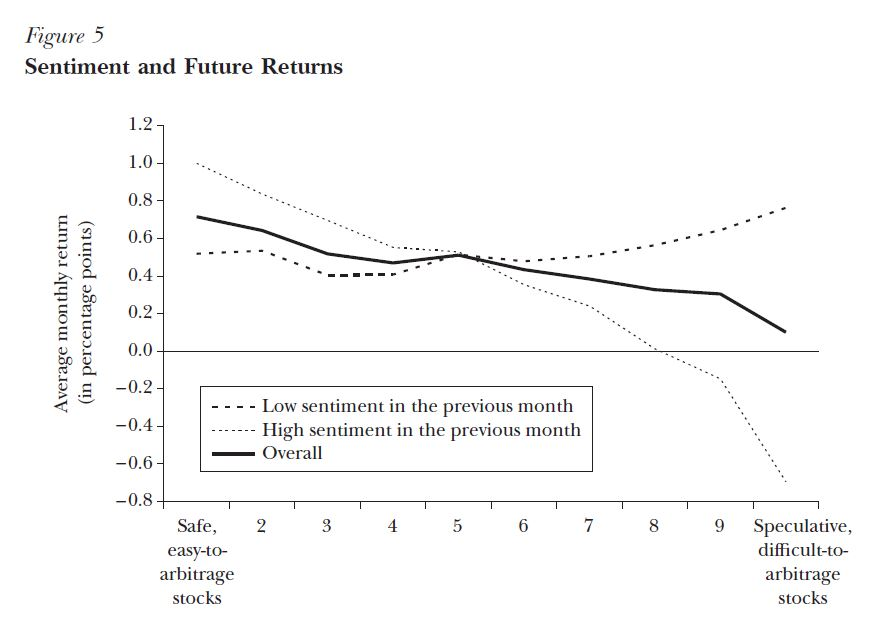
\includegraphics[width=0.50\textwidth]{figures/slide31_pic4.jpg}
\end{frame}

% --- Slide 32: Anomalies ---
\begin{frame}{Effects of Investor Sentiment on the Stock Market (III) --- Anomalies}
\begin{itemize}
\item Stambaugh, Yu, and Yuan (JFE 2012) argue that anomalies should be amplified following high sentiment
  \begin{itemize}
  \item The effect should concentrate on the short leg due to short-sale constraints
  \end{itemize}
\end{itemize}
\vfill
\centering
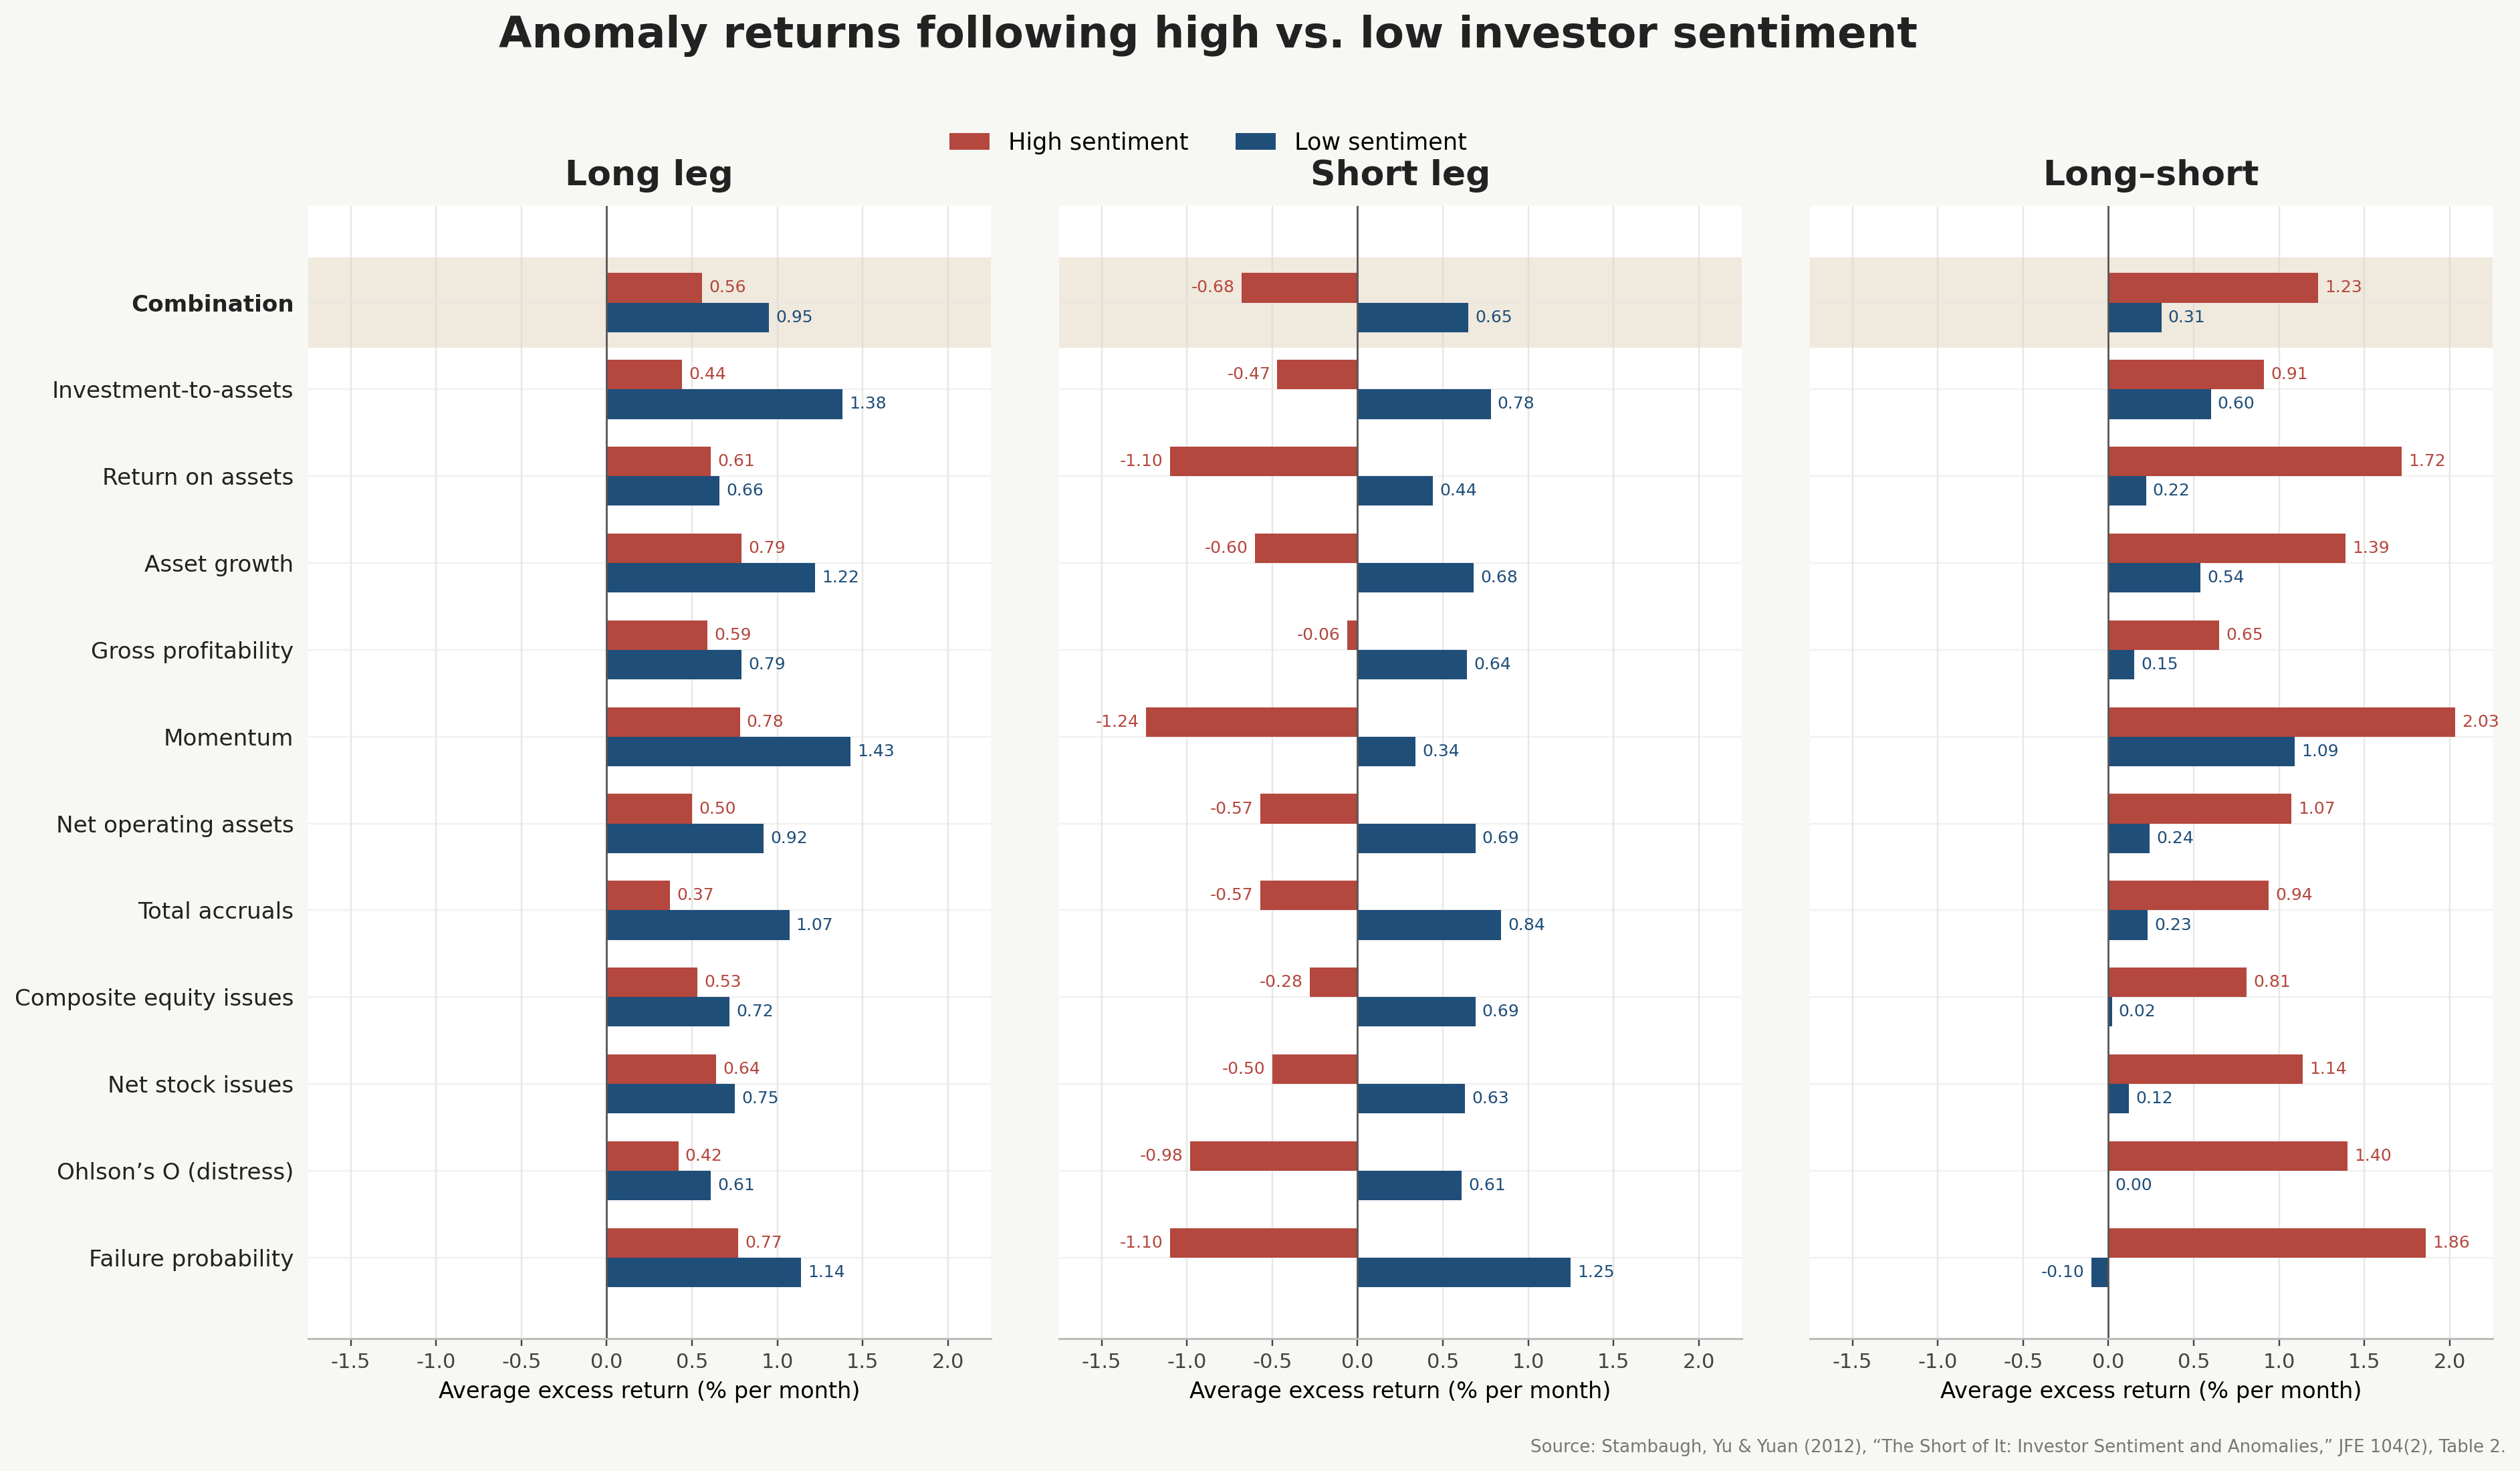
\includegraphics[width=0.55\textwidth]{figures/sentiment_anomaly.png}
\end{frame}

% --- Slide 33: Day of Week ---
\begin{frame}[shrink=5]{Effects of Investor Sentiment on the Stock Market (III) --- Anomalies, ctd.}
\begin{itemize}
\item Birru (JFE 2018) documents that long-short anomaly returns are strongly related to the day of the week
  \begin{itemize}
  \item In particular, long-short strategies earn the highest return on Monday and the lowest return on Friday; the effect concentrates in the short leg, which is more speculative
  \item Consistent with the psychology literature that mood increases (decreases) on Friday (Monday)
  \end{itemize}
\end{itemize}
\vfill
\centering
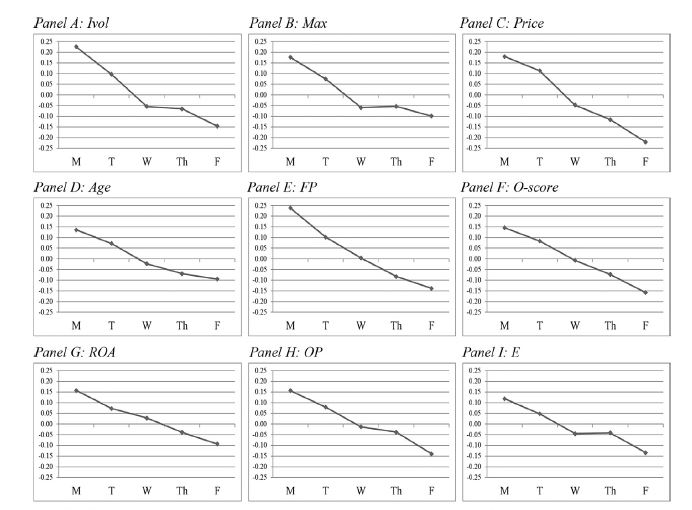
\includegraphics[width=0.45\textwidth]{figures/slide33_pic4.jpg}
\end{frame}


% --- Slide 34: Risk-Return Tradeoff ---
\begin{frame}[shrink=10]{Effects of Investor Sentiment on the Stock Market (IV) --- Risk-Return Trade-off}
\begin{columns}[T]
\begin{column}{0.50\textwidth}
\begin{itemize}
\item Shen, Yu, and Zhao (JME 2017) argue that sentiment also affects the cross-sectional risk-return trade-off
  \begin{itemize}
  \item When sentiment is high, sentiment-driven investors tend to require a smaller compensation for the risk they bear
  \item In addition, riskier stocks may be more subject to sentiment shifts and become more overpriced
  \item Coupled with short-sale constraints, the risk-return trade-off may be attenuated or even reversed during high sentiment periods
  \end{itemize} 
\end{itemize}
\end{column}
\begin{column}{0.45\textwidth}
\centering
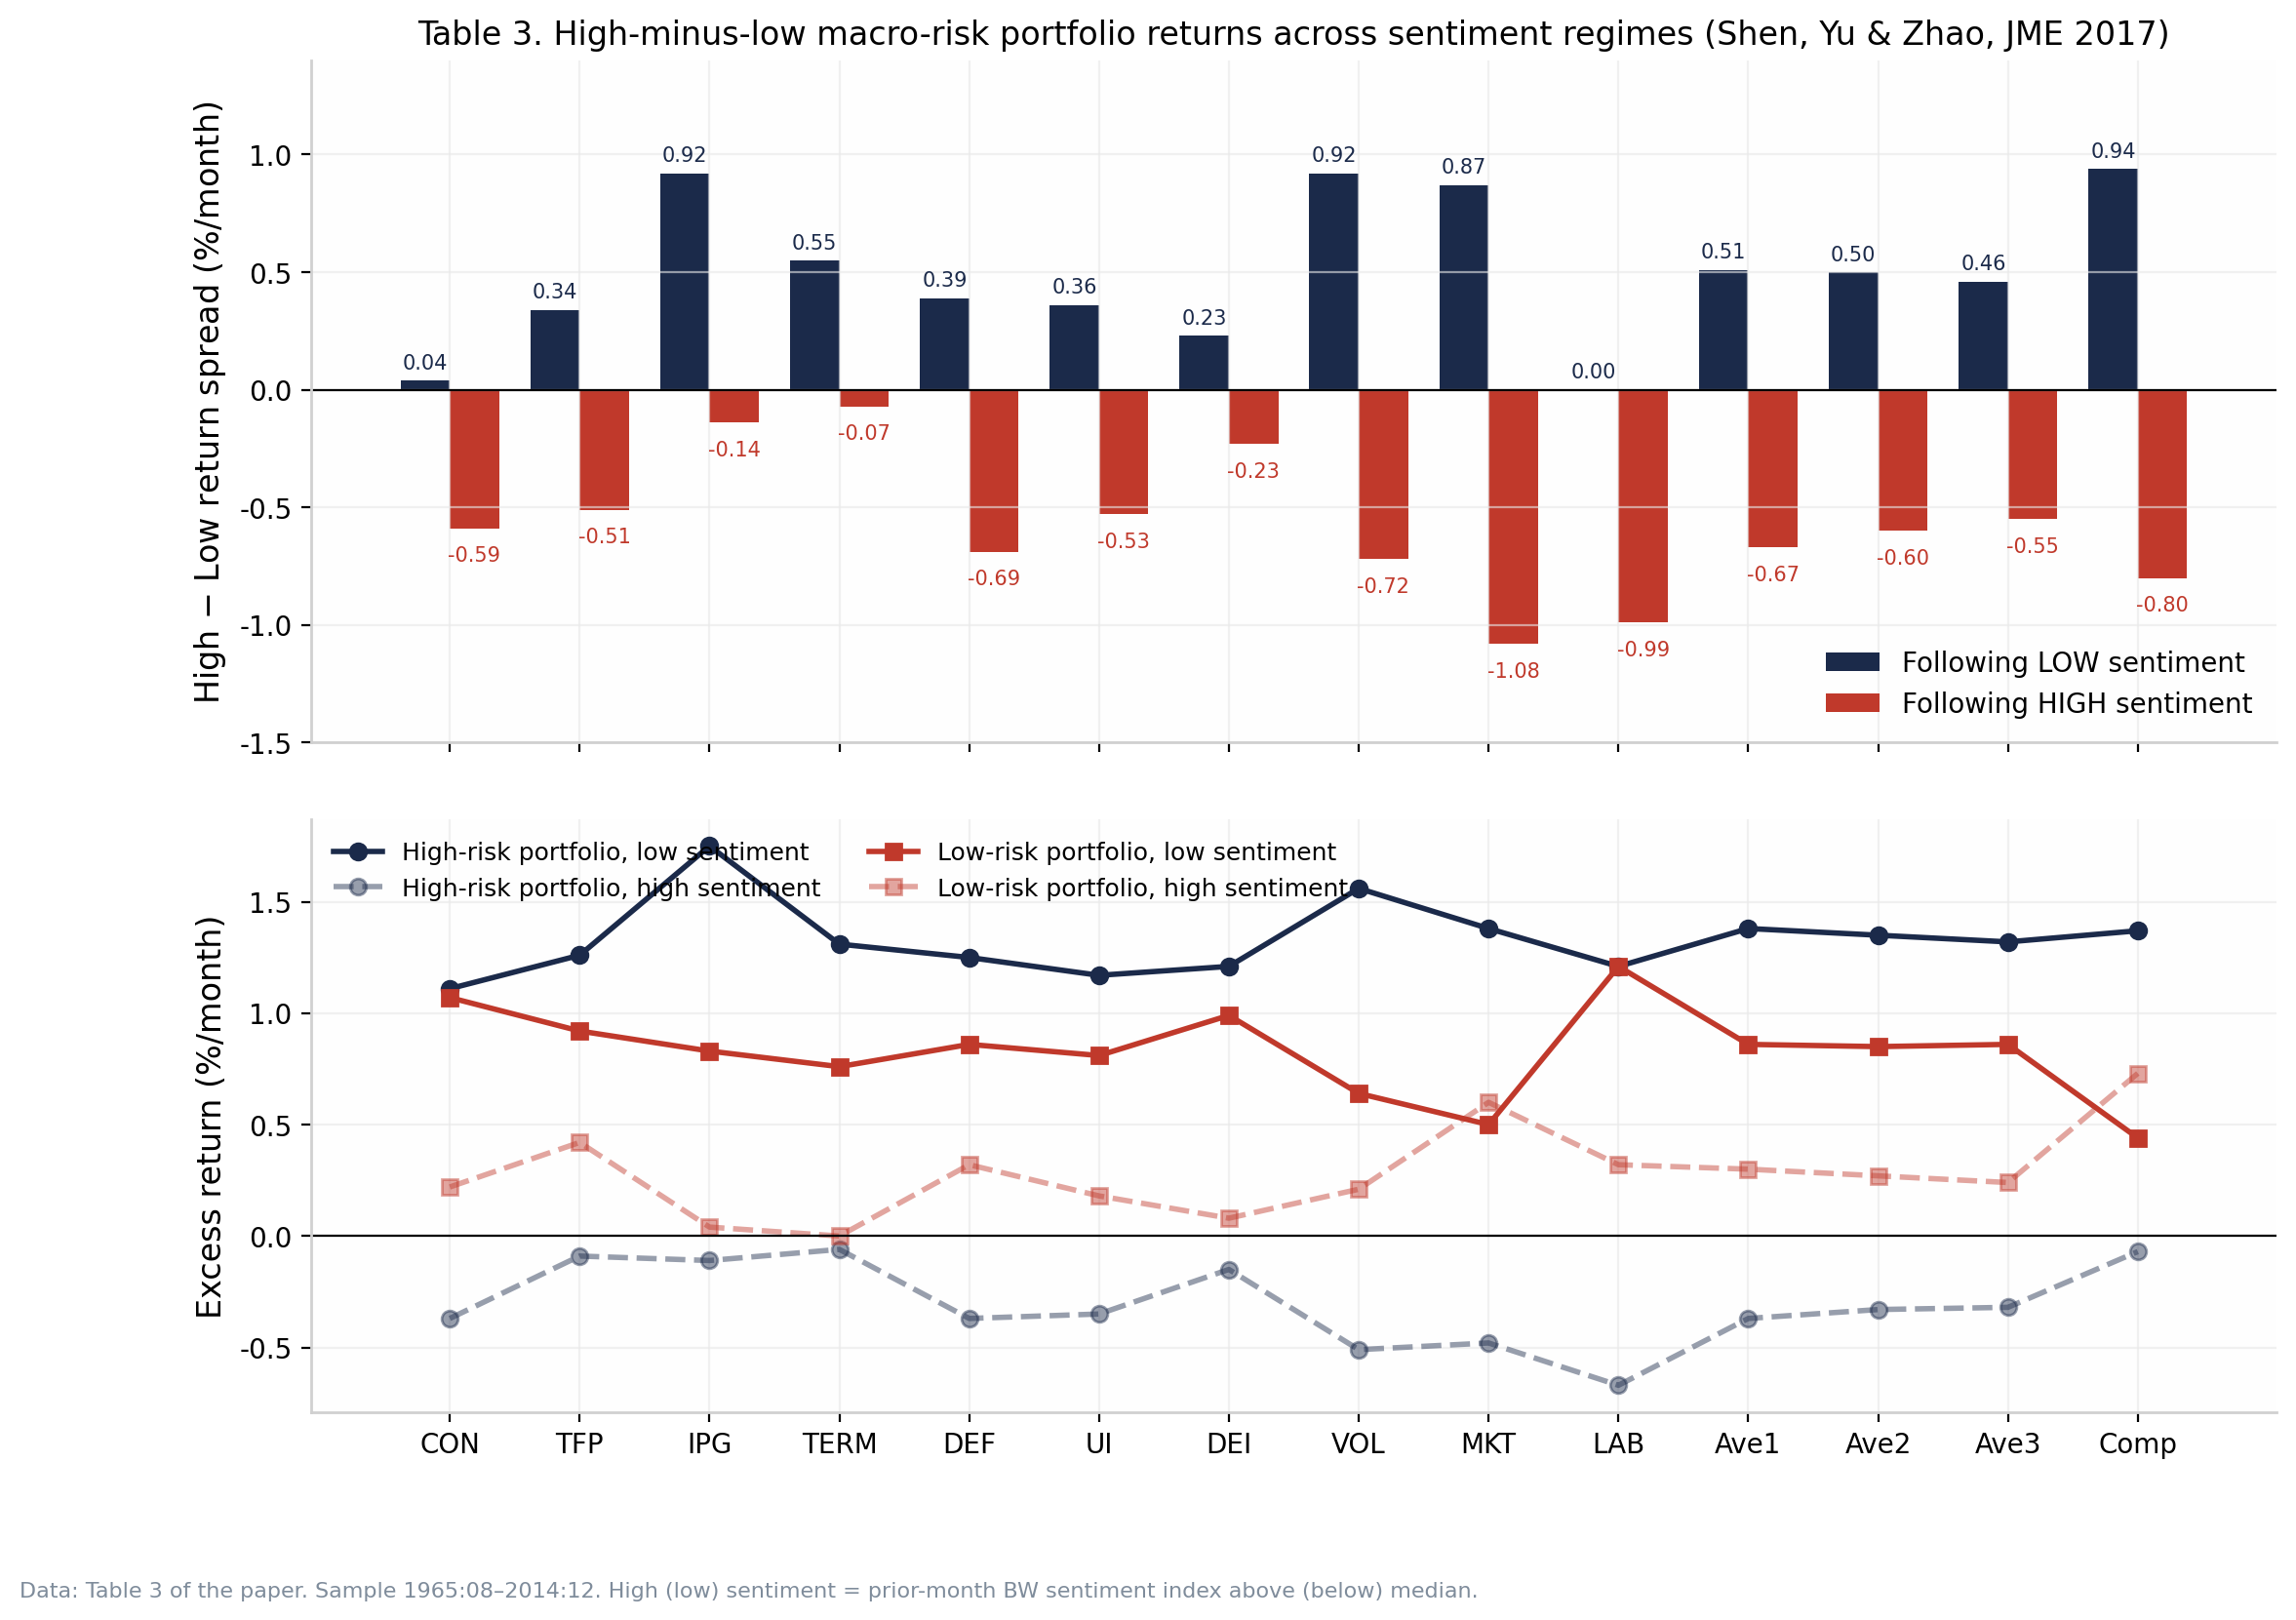
\includegraphics[width=\textwidth]{figures/sentiment_macrofactor.png}\\[0.2em]
\end{column}
\end{columns}
\end{frame}


% --- Slide 36: FEARS ---
\begin{frame}[shrink=10]{Other Measures of Aggregate Sentiment --- Google Search}
\begin{columns}[T]
\begin{column}{0.50\textwidth}
\begin{itemize}
\item Da, Engelberg, and Gao (RFS 2015)
\item Aggregate the volume of Google search queries related to household concerns and construct a Financial and Economic Attitudes Revealed by Search (FEARS) index as a new measure of investor sentiment
\item Benefits of FEARS:
  \begin{itemize}
  \item More transparent
  \item Higher frequency --- daily
  \item Reveal attitudes rather than inquire about them
  \end{itemize}
\item Gao, Ren, and Zhang (2020) document similar evidence for international markets
\end{itemize}
\end{column}
\begin{column}{0.48\textwidth}
\centering
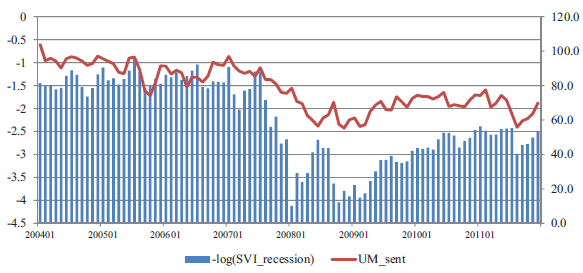
\includegraphics[width=\textwidth]{figures/slide36_pic4.png}
\begin{itemize}\small
\item FEARS is negatively related to contemporaneous returns
\item FEARS is positively related to future returns
\item FEARS predicts a temporary increase in volatility
\item FEARS predicts mutual fund flows out of equity funds to bond funds
\end{itemize}
\end{column}
\end{columns}
\end{frame}


% --- Slide 37: Manager Sentiment ---
\begin{frame}{Other Measures of Aggregate Sentiment --- Manager Sentiment}
\begin{columns}[T]
\begin{column}{0.50\textwidth}
\begin{itemize}
\item Jiang et al.\ (JFE 2019)
  \begin{itemize}
  \item Manager sentiment index based on the aggregated textual tone in 10-Ks, 10-Qs, and conference call transcripts
  \item Manager sentiment is a strong negative predictor of future aggregate stock market returns
  \end{itemize}
\end{itemize}
\end{column}
\begin{column}{0.48\textwidth}
\centering
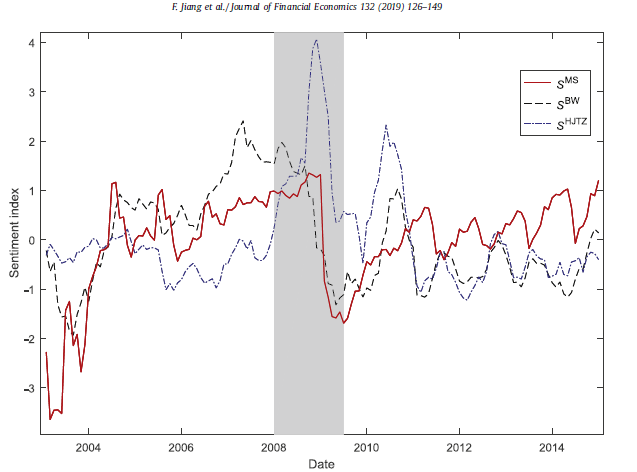
\includegraphics[width=\textwidth]{figures/slide37_pic4.png}
\end{column}
\end{columns}
\end{frame}

% --- Slide 38: Short Interests ---
\begin{frame}{Other Measures of Aggregate Sentiment --- Aggregate Short Interests}
\begin{columns}[T]
\begin{column}{0.50\textwidth}
\begin{itemize}
\item Short sellers are sophisticated investors who can correct mispricing induced by sentiment traders
\item Short interests aggregated to the market level are a strong contrarian predictor of future market returns
\end{itemize}
\end{column}
\begin{column}{0.48\textwidth}
\centering
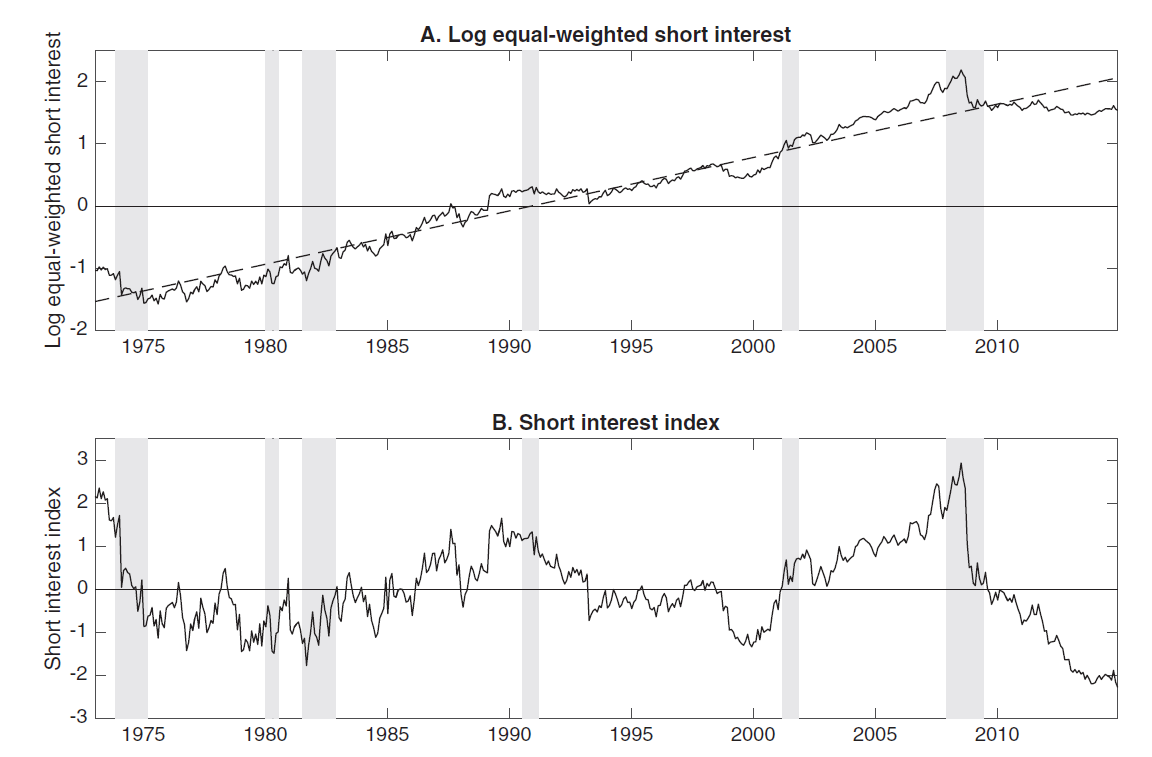
\includegraphics[width=\textwidth]{figures/slide38_pic4.png}
\end{column}
\end{columns}
\end{frame}

% --- Slide 39: Leveraged ETFs ---
\begin{frame}[shrink=5]{Other Measures of Aggregate Sentiment --- Flows to Leveraged ETFs}
\begin{columns}[T]
\begin{column}{0.50\textwidth}
\begin{itemize}
\item Leveraged ETFs provide amplified gains/losses to investors who bet on the direction of future market movement
\item Heavily traded and cater to speculative investors
\item Hence flows to such ETFs mainly reflect speculative investors' demand
\item Davies (2022) constructs a Speculative Sentiment Index (SSI) based on this insight
  \begin{itemize}
  \item SSI is the difference between share changes in the leveraged-long ETFs and share changes in the leveraged-short ETFs
  \end{itemize}
\item A 1-standard-deviation increase in the monthly index is associated with a 1.14\%--1.67\% decline in broad-market stock returns in the next month
\end{itemize}
\end{column}
\begin{column}{0.48\textwidth}
\centering
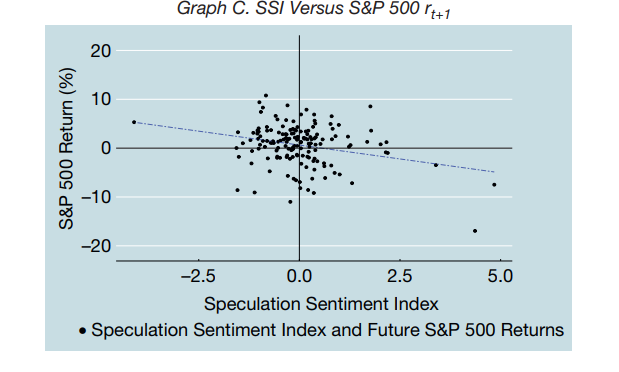
\includegraphics[width=\textwidth]{figures/slide39_pic5.png}
\end{column}
\end{columns}
\end{frame}

% --- Slide 40: Music Sentiment ---
\begin{frame}{Measuring Investor Mood/Emotions}
\begin{itemize}
\item Edmans et al.\ (2022): Music sentiment
\item The positivity of songs that individuals choose to listen to
\item \textbf{Advantages:}
  \begin{itemize}
  \item Real-time, continuous measure of national sentiment
  \item Language-free and comparable globally
  \item Exogenous to financial market events
  \end{itemize}
\item \textbf{Main findings:}
  \begin{itemize}
  \item Music sentiment is positively correlated with same-week equity market returns and negatively correlated with next-week returns
  \item Music sentiment also predicts increases in net mutual fund flows and precedes a rise in stock market volatility
  \item Negatively associated with government bond returns, consistent with a flight to safety
  \end{itemize}
\end{itemize}
\end{frame}

% --- Slide 41: Section ---
\section{Credit Market Sentiment}

\begin{frame}{}
\vfill
\centering
{\Large \textbf{Credit Market Sentiment}}
\vfill
\end{frame}

% --- Slide 42: Credit Sentiment Measure ---
\begin{frame}{Credit Market Sentiment}
\begin{itemize}
\item Greenwood and Hanson (RFS 2013) construct a sentiment measure for the credit market
  \begin{itemize}
  \item The idea is to compare the credit quality of high-issuance firms with that of low-issuance firms
  \item The insight is that a significant decline in issuers' credit quality is a reliable signal of credit market overheating
  \end{itemize}
\end{itemize}
\vfill
\centering
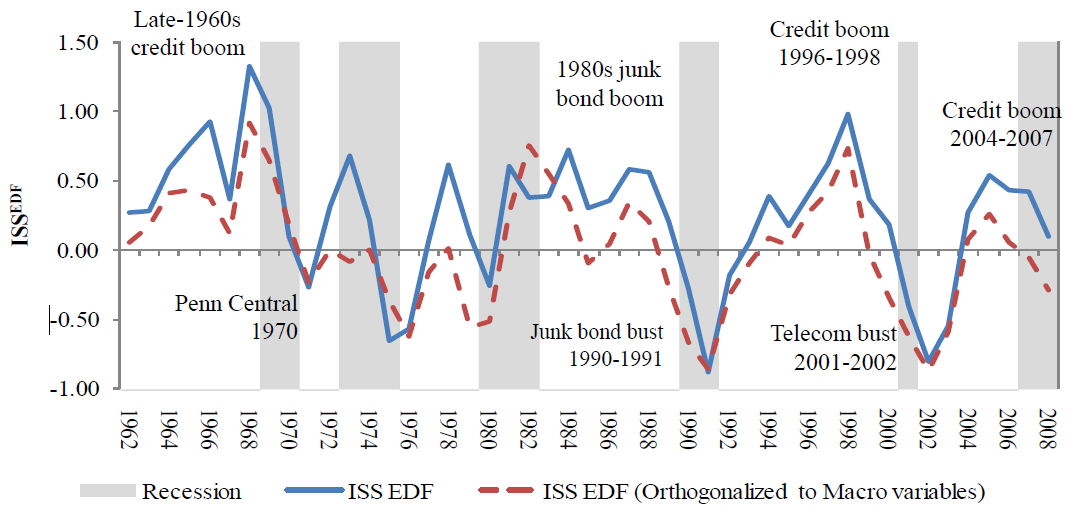
\includegraphics[width=0.55\textwidth]{figures/slide42_pic4.png}
\end{frame}

% --- Slide 43: Credit Sentiment Returns ---
\begin{frame}{Credit Market Sentiment Forecasts Excess Corporate Bond Returns}
\begin{itemize}
\item Economic magnitudes are significant:
  \begin{itemize}
  \item A 1-$\sigma$ increase in ISS EDF, the issuer expected default frequency, $\implies$ cumulative excess returns fall by 7.30\% over the following 2 years
  \end{itemize}
\end{itemize}
\vfill
\centering
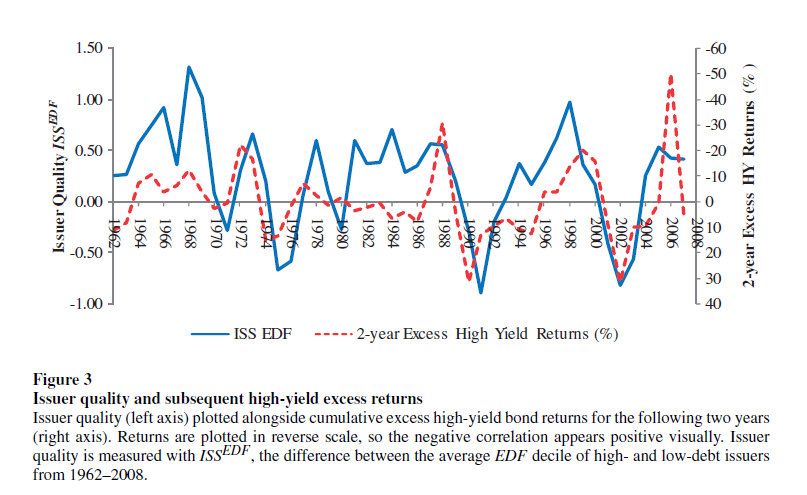
\includegraphics[width=0.55\textwidth]{figures/slide43_pic5.png}\\[0.2em]
\footnotesize Greenwood and Hanson (RFS 2013)
\end{frame}

% --- Slide 44: Credit and Growth ---
\begin{frame}{Credit Market Sentiment and Economic Growth}
\begin{columns}
\begin{column}{0.5\textwidth}
\begin{itemize}
\item Credit market overheating is associated with a higher probability of a future financial crisis and of economic downturns
  \begin{itemize}
  \item Schularick and Taylor (2012); Lopez-Salido, Stein, and Zakrajsek (2017); Baron and Xiong (2017)
  \end{itemize}
\end{itemize}
\end{column}
\begin{column}{0.48\textwidth}
\centering
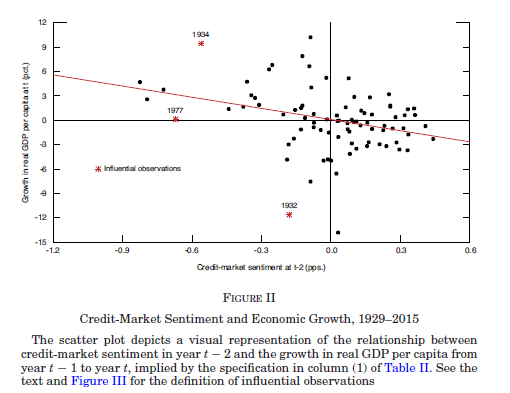
\includegraphics[width=\linewidth,height=0.75\textheight,keepaspectratio]{figures/slide44_pic4.png}\\[0.2em]
\footnotesize Lopez-Salido, Stein, and Zakrajsek (QJE 2017)
\end{column}
\end{columns}
\end{frame}

% --- Slide 45: Banking Crisis ---
\begin{frame}{Credit Expansion Predicts Banking Crises}
\begin{columns}
\begin{column}{0.5\textwidth}
\begin{itemize}
\item Baron and Xiong (QJE 2017) find bank credit expansion predicts increased bank equity crash risk
\item Despite the elevated crash risk, credit expansion predicts lower mean bank equity returns in the subsequent one to three years
\item Bank credit expansion is distinct from equity market sentiment captured by dividend yield
\item The result suggests overoptimism and neglect of crash risk by bank equity investors during credit expansions
\end{itemize}
\end{column}
\begin{column}{0.48\textwidth}
\centering
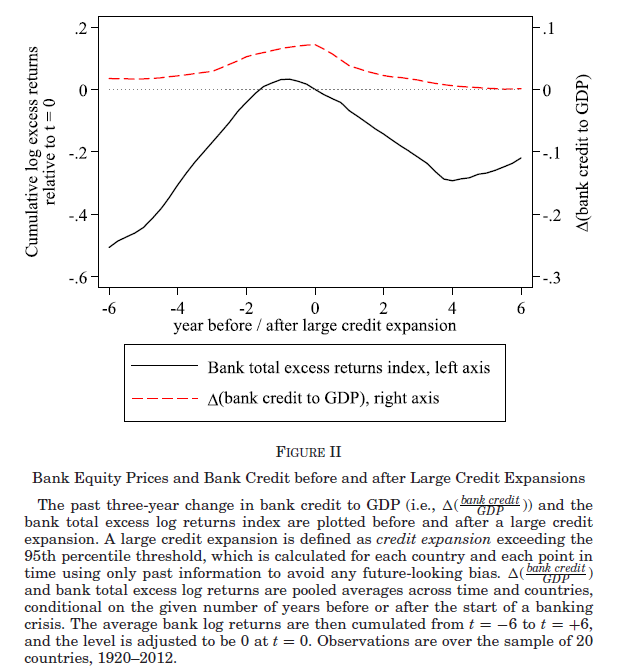
\includegraphics[width=\linewidth,height=0.75\textheight,keepaspectratio]{figures/slide45_pic4.png}\\[0.2em]
\footnotesize Baron and Xiong (QJE 2017)
\end{column}
\end{columns}
\end{frame}

% --- Slide 46: Predictable Crisis ---
\begin{frame}{Predictable Financial Crisis}
\begin{itemize}
\item Greenwood, Hanson, Shleifer, and Sorensen (JF 2022)
\item They use historical data on postwar financial crises around the world
\item The combination of rapid credit and asset price growth over the prior three years (R-zone) is associated with a 40\% probability of entering a financial crisis within the next three years
\end{itemize}
\vfill
\centering
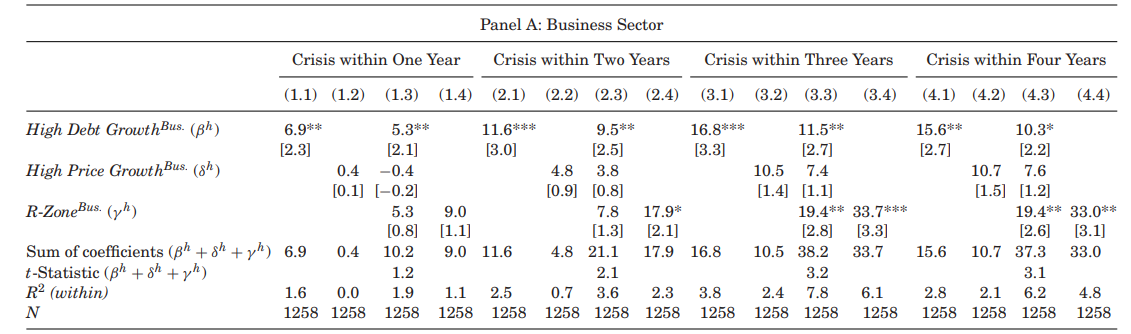
\includegraphics[width=0.70\textwidth]{figures/slide46_pic4.png}
\end{frame}

% --- Slide 47: Credit vs Equity Sentiment ---
\begin{frame}{Credit Market vs.\ Equity Market Sentiment}
\begin{itemize}
\item Empirical measures of credit market sentiment are only modestly correlated with measures of equity market sentiment
  \begin{itemize}
  \item Suggests we should not think of equity and credit markets as fully integrated
  \end{itemize}
\item Measures of expected returns on the stock market, such as Shiller's CAPE, do not predict future GDP growth (Lopez-Salido et al., 2017)
  \begin{itemize}
  \item Suggests credit market sentiment has potentially greater macroeconomic significance
  \end{itemize}
\end{itemize}
\end{frame}

% --- Slide 48: Determinants of Credit Sentiment ---
\begin{frame}{Narratives of the Credit Cycle}
\begin{itemize}
\item Short-term rates are low or have fallen in the recent past
  \begin{itemize}
  \item Push investors to ``reach for yield'' by buying bonds with longer duration and lower credit quality
  \end{itemize}
\item Term and credit spreads become compressed as a result
\item Default rates have been low or falling, because lower credit spreads allow low-quality firms to obtain cheap financing
\item This credit boom incentivizes low-quality firms to take on excessive leverage, making them vulnerable to even small external shocks
\item Consistent with empirical evidence on the boom-bust credit cycle
\end{itemize}
\end{frame}

% --- Slide 49: Early Indicator ---
\begin{frame}[shrink=5]{Early Indicator of the Credit Boom}
\begin{itemize}
\item Ben-Rephael, Choi, and Goldstein (JFE 2021)
\item Early indicator of credit boom based on intra-family flow shifts toward high-yield (HY) bond mutual funds
\item Intra-family flows likely capture investors' deliberate asset allocation decisions (rather than saving/investment decision)
\item It leads other indicators of the credit boom, such as growth in financial intermediary balance sheets, increases in shares of high-yield bond issuers, and downturns in various measures of credit spreads
\item Attributes the origins of the credit boom to an increase in investors' demand for HY bonds, perhaps due to biased perceptions of default risk
\end{itemize}
\vfill
\centering

\includegraphics[width=0.45\textwidth]{figures/slide49_pic4.png}
\end{frame}

% --- Slide 50: Behavioral Credit Cycle ---
\begin{frame}{A Behavioral Account of the Credit Cycle}
\begin{itemize}
\item Narrative of the credit cycle from Minsky's financial instability hypothesis and Kindleberger's \textit{Manias, Panics, and Crashes: A History of Financial Crises}
\item The full model is developed in Bordalo et al.\ (2018) and Greenwood, Hanson, and Jin (2024)
\item Key feature of the model is \textbf{reflexivity}: the feedback loop between investors' biased perceptions and market outcomes
\item \textbf{Main idea:}
  \begin{itemize}
  \item Investors hold extrapolative beliefs based on borrowers' recent default history
  \item During a boom, investors extend credit on attractive terms because borrowers have paid back in the past
  \item Even if borrowers' fundamental positions deteriorate, this may not be directly visible for a while because borrowers roll over debt at low rates
  \item When the reckoning eventually comes, markets overreact, slowing the recovery
  \end{itemize}
\end{itemize}
\end{frame}

% --- Slide 51: Summary ---
\begin{frame}{Summary}
\begin{itemize}
\item \textbf{Bounded rationality:}
  \begin{itemize}
  \item Limited attention leads to underreaction to news that is less salient or more costly to process
  \item Category thinking leads to excess return comovement
  \end{itemize}
\item \textbf{Psychology-free approaches:}
  \begin{itemize}
  \item Actions of sophisticated traders predict returns in the right direction
  \item Actions of noise traders negatively predict returns
  \item Investor sentiment predicts market returns and cross-sectional anomalies   
  \end{itemize}
\item \textbf{Credit market sentiment:}
  \begin{itemize}
  \item Distinct from equity market sentiment
  \item Predicts financial crises and economic downturns
  \item Behavioral models explain credit cycle dynamics
  \end{itemize}
\end{itemize}
\end{frame}

\end{document}
